\documentclass{beamer}

\usepackage{amsmath}
\usepackage{amssymb}
\usepackage{amsthm}
\usepackage{amsfonts}

\usepackage{hyperref}

\usepackage{tikz}
\usepackage{color}
\usetikzlibrary{calc,shapes,fadings}


\mode<presentation>
{
  \usetheme{Warsaw}
  \useoutertheme{mysplit}
}
% Remove the navigation bar
\setbeamertemplate{navigation symbols}{}

\graphicspath{{./imgs/}}

\title[Working with infinite posets]{Working with infinite posets}

\author{Damien Zufferey}

\institute{
  IST Austria (Institute of Science and Technology Austria)
}
\date{\today}

\begin{document}

% Title
\frame[plain]{\titlepage}

\begin{frame}
  \frametitle{Well-structured transition system}
  A well-structured transition system (WSTS)
  is a transition system $\langle S, \rightarrow, \leq \rangle$ such that:
  \begin{itemize}
  \item
    $\leq$ is a well-quasi-ordering (wqo),\\
    i.e. well-founded + no infinite antichain.
  \item
    compatibility of $\leq$ w.r.t. $\rightarrow$\\
    \begin{center}
    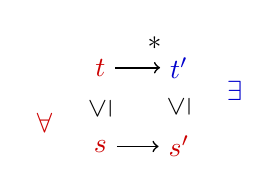
\begin{tikzpicture}[semithick, ->]
    \node[color=red!80!black] (s) {$s$};
    \node[color=red!80!black] (t) [above of=s] {$t$};
    \node[color=red!80!black] (sp) [right of=s] {$s'$};
    \node[color=blue!80!black] (tp) [right of=t] {$t'$};

    \path[color=white]  (s) edge node[color=black,rotate=90] {$\leq$} (t);
    \path  (s) edge (sp);
    \path  (t) edge node [above right] {*} (tp);
    \path[color=white]  (sp) edge node[color=black,rotate=90] {$\leq$} (tp);
    
    \node[color=blue!80!black] (exists) [above right of=sp] {$\exists$};
    \node[color=red!80!black] (forall) [below left of=t] {$\forall$};

    \end{tikzpicture}
    \end{center}
  \end{itemize}

  for more detail see: \cite{DBLP:journals/tcs/FinkelS01, DBLP:conf/lics/AbdullaCJT96}

\end{frame}

\begin{frame}
  \frametitle{Forward analysis of WSTS}
  %thomas illustration of post*
  \begin{center}
  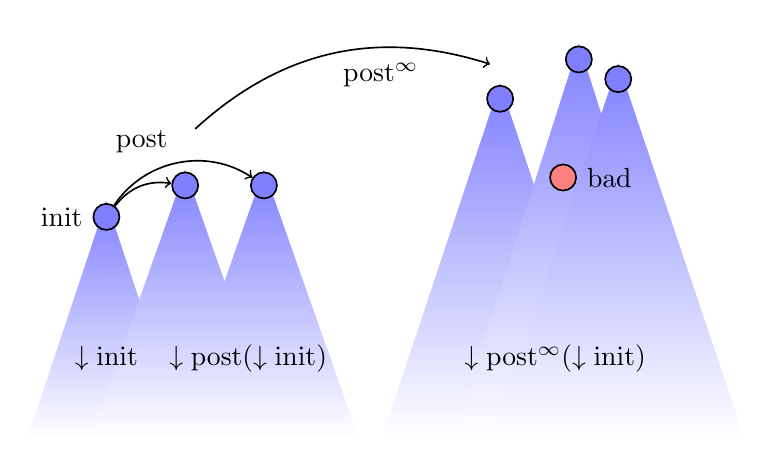
\begin{tikzpicture}[semithick,->]

  \shade[top color=blue!50,bottom color=white] (-3,-5) -- (-4,-2) -- (-5,-5);
  \node[draw,circle,fill=blue!50,minimum height=0.2,label={left:init}] (e1) at (-4,-2.2) {};

  \shade[top color=blue!50,bottom color=white] (-1.8,-5) -- (-3,-1.6) -- (-4.2,-5);
  \node[draw,circle,fill=blue!50,minimum height=0.2] (e2) at (-3,-1.8) {};
  \shade[top color=blue!50,bottom color=white] (-0.8,-5) -- (-2,-1.6) -- (-3.2,-5);
  \node[draw,circle,fill=blue!50,minimum height=0.2] (e3) at (-2,-1.8) {};
  \path (e1) edge[bend left] (e2);
  \path (e1) edge[bend left=45] node[above left] {post} (e3);
  \node at (-2.2,-4) {$\downarrow\text{post}(\downarrow\text{init})$};

  \shade[top color=blue!50,bottom color=white] (2.5,-5) -- (1,-0.5) -- (-0.5,-5);
  \node[draw,circle,fill=blue!50,minimum height=0.2] at (1,-0.7) {};
  \shade[top color=blue!50,bottom color=white] (3.6,-5) -- (2,0) -- (0.4,-5);
  \node[draw,circle,fill=blue!50,minimum height=0.2] at (2,-0.2) {};
  \shade[top color=blue!50,bottom color=white] (4.1,-5) -- (2.5,-0.25) -- (0.9,-5);
  \node[draw,circle,fill=blue!50,minimum height=0.2] at (2.5,-0.45) {};

  \node (e4) at (-3,-1.2) {};
  \node (e5) at (1,-0.3) {};
  \path (e4) edge[bend left] node[below right] {post$^\infty$} (e5);
  \node at (1.7,-4) {$\downarrow\text{post}^\infty(\downarrow\text{init})$};

  \node[draw,circle,fill=red!50,minimum height=0.2,label={right:bad}] at (1.8,-1.7) {};
  %on top of the shades
  \node at (-4,-4) {$\downarrow\text{init}$};
  \end{tikzpicture}
  \end{center}
\end{frame}

\begin{frame}{Understanding what happens in \emph{post$^\infty$}}
Computing \emph{post$^\infty$} should not take $\infty$ steps. Therefore, \alert{acceleration} is used.

\vspace{10pt}

Given a sequence of transitions as a function $f$, we need to be able to compute $f^\infty(x)$.
Also know as the \emph{least upper bound acceleration} of $f$.

\vspace{10pt}

\begin{block}{Problem}
The analysis converges only if the system has a finite number of \emph{behaviours}, i.e. there is a finite number of acceleration to compute.
This condition is also known as \alert{flattability}.
Acceleration is path dependent.
\end{block}

\vspace{10pt}

In practice, finding all the sequences to accelerate (complete algorithm) is already prohibitively expansive.

\end{frame}

\begin{frame}{An analysis that does not depend on the paths ?}
  \begin{block}{Idea}
    Forcing the termination of the analysis by having an analysis that is not path dependent (e.g. abstract interpretation) at the cost of precision.
  \end{block}

  \vspace{10pt}

  As an abstract domain, we can use the set of downward-closed sets (+ ideal completion), like the usual analysis.
  But the acceleration is replaced by \alert{widening} ($\nabla$).
  
  \vspace{10pt}

  Quick reminder, $\nabla$ \cite{CousotCousot77AbstractInterpretation}:\\
  for every infinite sequence $s_0, s_1, \ldots$ the sequence $C_0, C_1, \ldots$, where $C_0 = s_0, C_i = C_{i-1} \nabla s_i$, is not strictly increasing.

  \vspace{10pt}

  Hence, the termination of the analysis relies only on the properties of the \alert{underlying space}, not the transitions.

\end{frame}

\begin{frame}{What are we looking for ?}

Goal: a good widening operator that is as general as possible.

\vspace{10pt}

Idea: jumping to the limit of ascending chains.

\vspace{10pt}

Problem: proving that this is actually a widening oprator.

\vspace{10pt}

Thus, we need to understand the \alert{structure} of $S$.

\vspace{10pt}

Try to get a feeling of what is this structure by following:
\begin{block}{\cite{DiestelPikhurko03FactoringPoset}}
\centering
On the cofinality of infinite partially ordered sets:\\
factoring a poset into lean essential subsets
\end{block}

\end{frame}

\begin{frame}{Example: acceleration for Petri net}

Assumes we have a Petri net with 4 places.
The state space is $\mathbb{N}^4$.
After adding limit elements we get $\mathbb{N}^4_\infty$.

\vspace{10pt}

Let $t$ be a sequence of transitions s.t. $(1,0,1,0) \rightarrow_t (2,1,1,0)$.\\
acceleration gives: $\bigcup_{i=0}^\infty \rightarrow_t^i((1,0,1,0)) ~ = ~ \downarrow (\infty, \infty, 1, 0)$

\vspace{10pt}

In this case a widening operator compares two state $a,b$, checks that $a \leq b$, and sets to $\infty$ every component that is stricly greater in $b$.

\vspace{10pt}

Can we generalize this approach to a more general setting ?

\end{frame}


\begin{frame}{Definitions (1)}
  
\begin{itemize}
\item A \emph{quasi-order} (preorder) in a reflexive and transitive relation.
\item A \emph{partial order} is a reflexive, transitive, and anti-symmetric relation.
\item A \emph{well-quasi-order} is a quasi-order that has no infinite antichain or infinite strictly decreasing sequence.
\item $\uparrow x = \{ x' \in S \,|\, x \leq x' \}$ is an upward-closed set.
\item $\downarrow x = \{ x' \in S \,|\, x' \leq x \}$ is an downward-closed set.
\end{itemize}

  \vspace{10pt}

Why using quasi order rather than partial order:\\
\mbox{}~~Because anti-symmetry is not needed for the proofs.\\
\mbox{}~~In practice, most of the quasi-orders used are partial orders.

\begin{block}{Hypothesis}
Let $S$ be an infinite (but countable) partially ordered set (poset).
\end{block}

\end{frame}

\begin{frame}{Definitions (2)}

\begin{itemize}
\item A \emph{chain} is totally ordered subset of $S$.
\item A \emph{directed} set $D$ is a set such that $\forall x,y \in D, ~ \exists z \in D, ~ x \leq z \land y \leq z$.
\item $P \subseteq S$ is \emph{cofinal} iff $\downarrow P = S$.
\item $P \subseteq S$ is \emph{small} iff it is not cofinal.
\item The \emph{cofinality} of $S$, denoted cf($S$), is the least cardinality of the cofinal subset of $S$.
\item $P$ is \emph{lean} iff all $Q \subseteq P$ with $|Q| > \text{cf}($P$)$ are cofinal.
\item $P$ is \emph{divisible} iff it is the union of fewer than cf($P$) small subsets.
\item $P \subseteq S$ is \emph{essential} iff it is the complement of a small set.
\end{itemize}

\begin{block}{Hypothesis}
$\text{cf}(S) = \aleph_0$. (infinite but countable)
\end{block}

\end{frame}

\begin{frame}{About directed sets}

Why are directed sets important ?\\
\mbox{}~~~~They generalize chains and\\
\mbox{}~~~~acceleration ($\bigcup_{i=0}^\infty f^i(x)$) generates an ascending chain.

\vspace{10pt}

\begin{block}{$P$ is directed iff $P$ contains a cofinal chain $C$.}
$\Leftarrow$: a chain is directed.\\
$\Rightarrow$: build a chain by enumerating $P$ and taking the lub.
\end{block}

\vspace{10pt}

\begin{block}{$P$ is directed iff $P$ is not a union of two small subsets.}
$\Leftarrow$: assume $P$ is not directed, pick two elements without upper bounds, use them to create a partition.\\
$\Rightarrow$: assume $P$ is the union of two small subsets, what about the lub of the elements in those subset ?
\end{block}

\vspace{10pt}

Indivisible posets are directed.

\end{frame}

\begin{frame}{Directed sets and lean sets}

Why lean sets ? What do they represents ?\\
\mbox{}~~~~ A lean set do not contains too much ``garbage''.

\vspace{10pt}

\begin{block}{$P$ is directed iff $P$ contains a lean equivalent subset.}
$\Rightarrow$: we know $P$ contains a cofinal chain and chains are lean.\\
$\Leftarrow$: lean sets are indivisible, equivalent sets share divisibility.
\end{block}

\vspace{10pt}

For subsets $P$ of $S$, the following statements are equivalent:
\begin{itemize}
\item $P$ is directed;
\item $P$ is indivisible;
\item $P$ has a cofinal chain;
\item $P$ has a lean equivalent subset.
\end{itemize}

\end{frame}

\begin{frame}{Factoring posets into essential directed subset}

We need one more concept: \emph{essential} subset.\\
\mbox{}~~~~An essential subset is the complement of a small subset.\\
\mbox{}~~~~Hence, $P \not\leq P \setminus B$ and $B \not\leq P \setminus B$

\vspace{10pt}

Let $\bigcup_{i < \text{cf}(S)} A_i$ be a partition of $S$ into \emph{essential directed subsets}.

\vspace{10pt}

\begin{block}{Every essential directed subset of $S$ is equivalent to some $A_j$}
Let $B$ be an essential directed subset of $S$.
Define $B_i = B \cap A_i$.
Because $B$ is directed (indivisible) there is $j$ s.t. $B \leq B_j \subseteq A_j$.\\
If $A_j \leq B$ we are done.
Otherwise, $B$ is small in $A_j$ which implies $(B \leq) A_j \leq A_j \setminus B_j (\subseteq P \setminus B)$.
This contradicts that $B$ is essential.
\end{block}

\end{frame}

\begin{frame}{What about our original space a WQO ?}

\begin{block}{If $S$ is well-quasi-ordered, it admits a partition into fewer than cf($S$) indivisible (essential) subsets.}
See \cite{Diestel01RelatingSubsetsOfAPoset} for the proof.
\end{block}

\end{frame}

\begin{frame}{What about our widening operator ?}

Widening generates indivisible directed subsets, but not essential.

\vspace{10pt}

What can we do ?

\vspace{10pt}

\begin{block}{Theorem by \cite{Pouzet80antichains}}
Every directed poset $S$ without infinite antichains has a cofinal subsets that is isomorphic to the direct product of finitely many distinct regular cardinals, the largest of which is cf($S$).
\end{block}

\vspace{10pt}

Direct product ? ~~ like the case of Petri nets.\\
Regular cardinals ? ~~ ...

\vspace{10pt}

The hope it to prove that the widening is taking the limit of one of the component of the directed product.

\end{frame}

\iffalse
\begin{frame}
  \frametitle{Adequate Domain of Limit (1)}
  ADL: \cite{GeeraertsETAL06ExpandEnlargeCheck}\\
  let $Y$ an ADL for wqo set $X$:
  \[\text{For every} ~ z \in \text{X} \cup \text{Y}, \gamma(z) ~ \text{is a downward-closed subset of X}.\]

  \begin{center}
  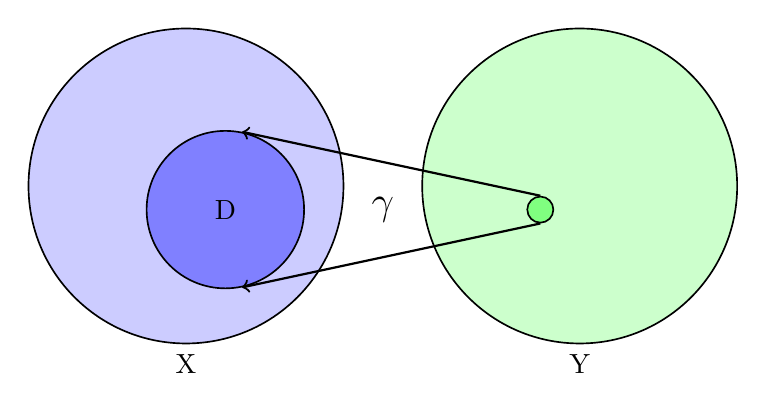
\begin{tikzpicture}[semithick, ->]
  \node [draw,circle,fill=blue!20, minimum height=4cm, label={below:X}] at ( -2.5, 0) {};
  \node [draw,circle,fill=green!20, minimum height=4cm, label={below:Y}] at ( 2.5, 0) {};
  
  \node [draw,circle,fill=green!50] (a) at ( 2, -0.3) {};
  \node [draw,circle,fill=blue!50, minimum height=2cm] (b) at ( -2, -0.3) {D};
  \draw[thick] (a.north) -- (tangent cs:node=b,point={(a.north)},solution=1);
  \draw[thick] (a.south) -- (tangent cs:node=b,point={(a.south)},solution=2);
  \node at ( 0, -0.3) {\Large $\gamma$};

  \end{tikzpicture}
  \end{center}
\end{frame}

\begin{frame}
  \frametitle{Adequate Domain of Limit (2)}
  \begin{center}
    Every downward-closed subset D of X is\\
    generated by a finite subset E of Y $\cup$ X.
  \end{center}

  \begin{center}
  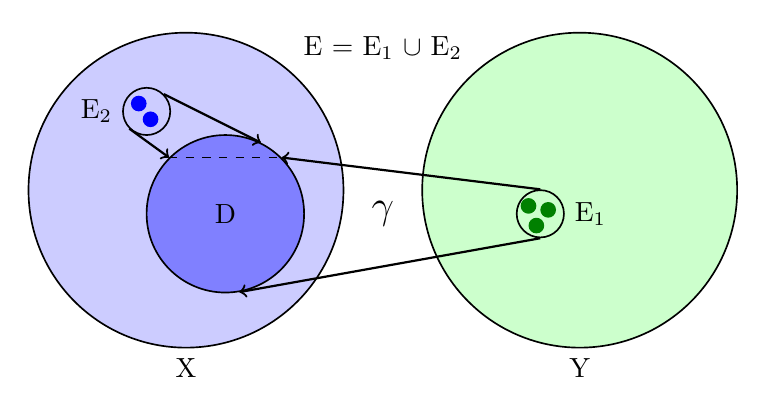
\begin{tikzpicture}[semithick]
  \node [draw,circle,fill=blue!20, minimum height=4cm, label={below:X}] at ( -2.5, 0) {};
  \node [draw,circle,fill=green!20, minimum height=4cm, label={below:Y}] at ( 2.5, 0) {};
  
  \node [draw,circle,minimum height=6mm,label={right:E$_1$}] (a) at ( 2, -0.3) {};
  \node[circle,fill=green!50!black,inner sep=2pt] at (2.1, -0.25) {};
  \node[circle,fill=green!50!black,inner sep=2pt] at (1.95, -0.45) {};
  \node[circle,fill=green!50!black,inner sep=2pt] at (1.85, -0.2) {};
  \node [draw,circle,fill=blue!50, minimum height=2cm] (b) at ( -2, -0.3) {D};
  \draw[dashed] (b.north west) -- (b.north east);
  \draw[thick,->] (a.north) -- (b.north east);
  \draw[thick,->] (a.south) -- (tangent cs:node=b,point={(a.south)},solution=2);
  \node at ( 0, -0.3) {\Large $\gamma$};
  
  \node at ( 0, 1.8) {E = E$_1$ $\cup$ E$_2$};

  \node [draw,circle,minimum height=6mm,label={left:E$_2$}] (c) at ( -3, 1) {};
  \node[circle,fill=blue,inner sep=2pt] at (-3.1, 1.1) {};
  \node[circle,fill=blue,inner sep=2pt] at (-2.95, 0.9) {};
  \draw[thick,->] (c.north east) -- (tangent cs:node=b,point={(c.north east)},solution=2);
  \draw[thick,->] (c.south west) -- (b.north west);


  \end{tikzpicture}
  \end{center}
\end{frame}

\begin{frame}{Sober and Noetherian Spaces}
%TODO
\end{frame}
\fi

\begin{frame}[allowframebreaks]{References}
  \frametitle{}
  {\tiny
  %\bibliographystyle{annotate}
  %\bibliographystyle{plainnat}
  \bibliographystyle{cell}
  %\bibliographystyle{abbrvnat}
  \bibliography{biblio}
  }
\end{frame}

\end{document}
